\appendix
\section*{\Huge Supplemental Material}

\setcounter{section}{0}

% https://tex.stackexchange.com/a/708552/316176
\makeatletter
\def\@seccntformat#1{\@ifundefined{#1@cntformat}%
   {\csname the#1\endcsname\space}%    default
   {\csname #1@cntformat\endcsname}}%  enable individual control
\newcommand\section@cntformat{\thesection.\space} % section-level
\makeatother
\renewcommand{\thesection}{S\arabic{section}}
\counterwithin{equation}{section}
\counterwithin{figure}{section}
\counterwithin{table}{section}
\counterwithin{theorem}{section}
\counterwithin{algorithm}{section}
\counterwithin{lstlisting}{section}

\vspace{0.8em}

Below is supplemental material for our paper \citep{supplemental} with discussions and figures that were not put in the main paper.

\subsection{Algorithm Equivalency}

\label{sec:algorithm:equivalency}

We shall demonstrate the accuracy of the proposed shortcut algorithm by providing a proof overview of how it is equivalent to the old algorithm (and assuming the old algorithm is a `good' reconstruction algorithm).
We define `equivalent' in this context to mean that every node at which an organism can be placed by the naive algorithm is also a node at which one can be placed by the shortcut algorithm (i.e. the shortcut algorithm places nodes at points that the naive algorithm could, given the right arbitrary choices).

%Consider adding some organism $o$ to the reconstructed tree $T$, which follows exactly one of the following cases: there is no missing information (i.e., $\forall (r, d) \in o\ r = \operatorname{rank}(\operatorname{children}(n))$, where $n$ is the current node throughout iteration), or there is.
The case where there is no missing information is trivial -- the only difference between the original and new algorithm lies when there is missing information, the absence of which rendering them the same.

Therefore, consider analyzing data at rank $r$ and having some missing information between the $\operatorname{rank}(n)$ and $r$.
Now, consider cases on whether there is some successive path of matching differentiae:

%\begin{itemize}
%  \item \textbf{There is some path.}
%  Therefore, we know that this path contains a descendant $n'$ of $n$ with rank $r$ and differentia $d$.
%  In the naive algorithm, this descendant is select to be the next $n$ when processing the information of $o$, as the optimal path found includes $n'$.
%  However, we also know that the shortcut algorithm must have created a shortcut from $n$ to $n'$ (and possibly collapsed it with other valid descendants, which is irrelevant as the path still remains).
%  So, the shortcut algorithm (in line 10 of the naive Algorithm~\ref{alg:old} as described in the paper) finds this child and selects it to be the new $n$ as well.
%  \item \textbf{There is no such path.}
%  Since there is no candidate path to follow, the naive algorithm simply creates a new node branching off $n$ with rank and differentia $(r, d)$.
%  Then, this new node is made the new $n$.
%  Since there was no valid path, we see that $n$ has no descendants with rank $r$ and differentia $d$.
%  Therefore, there is no shortcut built from $n$ to such a node, as it does not exist.
%  So, the shortcut algorithm will also branch off of $n$ by creating a new node in the same manner as the naive one.
%\end{itemize}

In either case, we have shown that both algorithms make effectively the same decisions when it comes to selecting nodes $n$ throughout each iteration of \textsc{TreeInsert}.
Because original relationships between nodes are still preserved, choosing a particular node to branch off of conveys identical information in both algorithms.
In conclusion, the two algorithms are equivalent in correctness.
However, it is worth noting that in cases where multiple paths are valid, the algorithms may make different decisions (as the chosen path out of these is arbitrary) and therefore may not be exactly equivalent.

\subsection{Algorithm Implementations}

The shortcut-based algorithm is implemented in the \texttt{hstrat} Python package \citep{moreno2022hstrat} as \texttt{hstrat.build\_tree\_searchtable}.
The reconstruction backend is selectable between independent implementations written in either pure Python or in C++, bound via Pybind11 \citep{wenzel2017pybind11}.
Benchmarks comparing the shortcut-enabled approaches to the existing naive approach, implemented in pure Python, used the pure Python backend for the shortcut-enabled approach, to ensure apples-to-apples comparability.
Other benchmarking and validation experiments used the C++ backend, which is expected to be better reflective of how the library will be used in practice, given the inherent speedup and memory savings associated with compiled code.

As suggested by the function name, both shortcut-enabled backends represent trie data using an edge-list table, rather than a node-and-pointer approach, as is the case with the existing naive implementation.
From an algorithmic perspective, tabular and node-and-pointer data structures provide identical properties for traversal and lookup operations.
However, in practice, the former approach is often faster due to fewer memory allocation operations and better cache locality.

At the implementation level, we represent trie shortcuts via additional columns in our edge table.
When a new node is appended, its shortcut edge is initialized identically to its trie edge.
From this point onwards, shortcut edges are used only for traversing the trie, while underlying trie edges --- treated as immutable from node initialization onwards --- are used when reading out the final reconstruction result.

\subsection{Build-time Garbage Collection}

To reduce memory usage for very large phylogeny reconstructions, we supplement the core trie extension and consolidation procedure detailed in Section~\ref{sec:algorithm} with an intermittent garbage collection step.
Because genomes are inserted in ascending order of generational depth, trie nodes at a generation with a single child node.
Given that all trie nodes only have a single parent node, such a ``dropped unifurcation node'' can be excised and safely replaced with an edge directly connecting its parent and child.

As currently implemented, we use the presence of modifications to shortcut edges to identify nodes for which corresponding hstrat markers have been dropped.
We note that this does not detect all dropped unifurcations, and an alternate more aggressive approach could be implemented readily by incorporating information as to which markers have been dropped from the marker retention algorithm used at runtime.

At implementation-level, the frequency of ``dropped unifurcation'' garbage collection is provided as a configurable function parameter, and so can be tuned as appropriate for a given use case scenario.
Garbage collection was not necessary for the up to 10 million tip reconstructions evaluated in our microbenchmarking experiment, and so was not performed.
For our macrobenchmark experiments, we ran this procedure at three evenly-spaced intervals during the build process.
Figure~\ref{fig:billion-tip-time} details the share of net execution time consumed by purging dropped unifurcations in these trials.

\subsection{Validation with Ground Truth}

In addition to determining triplet distance between ground truth and reconstructed phylogenies, we ran visualizations to make comparisons more interpretable.

\begin{figure}[h]
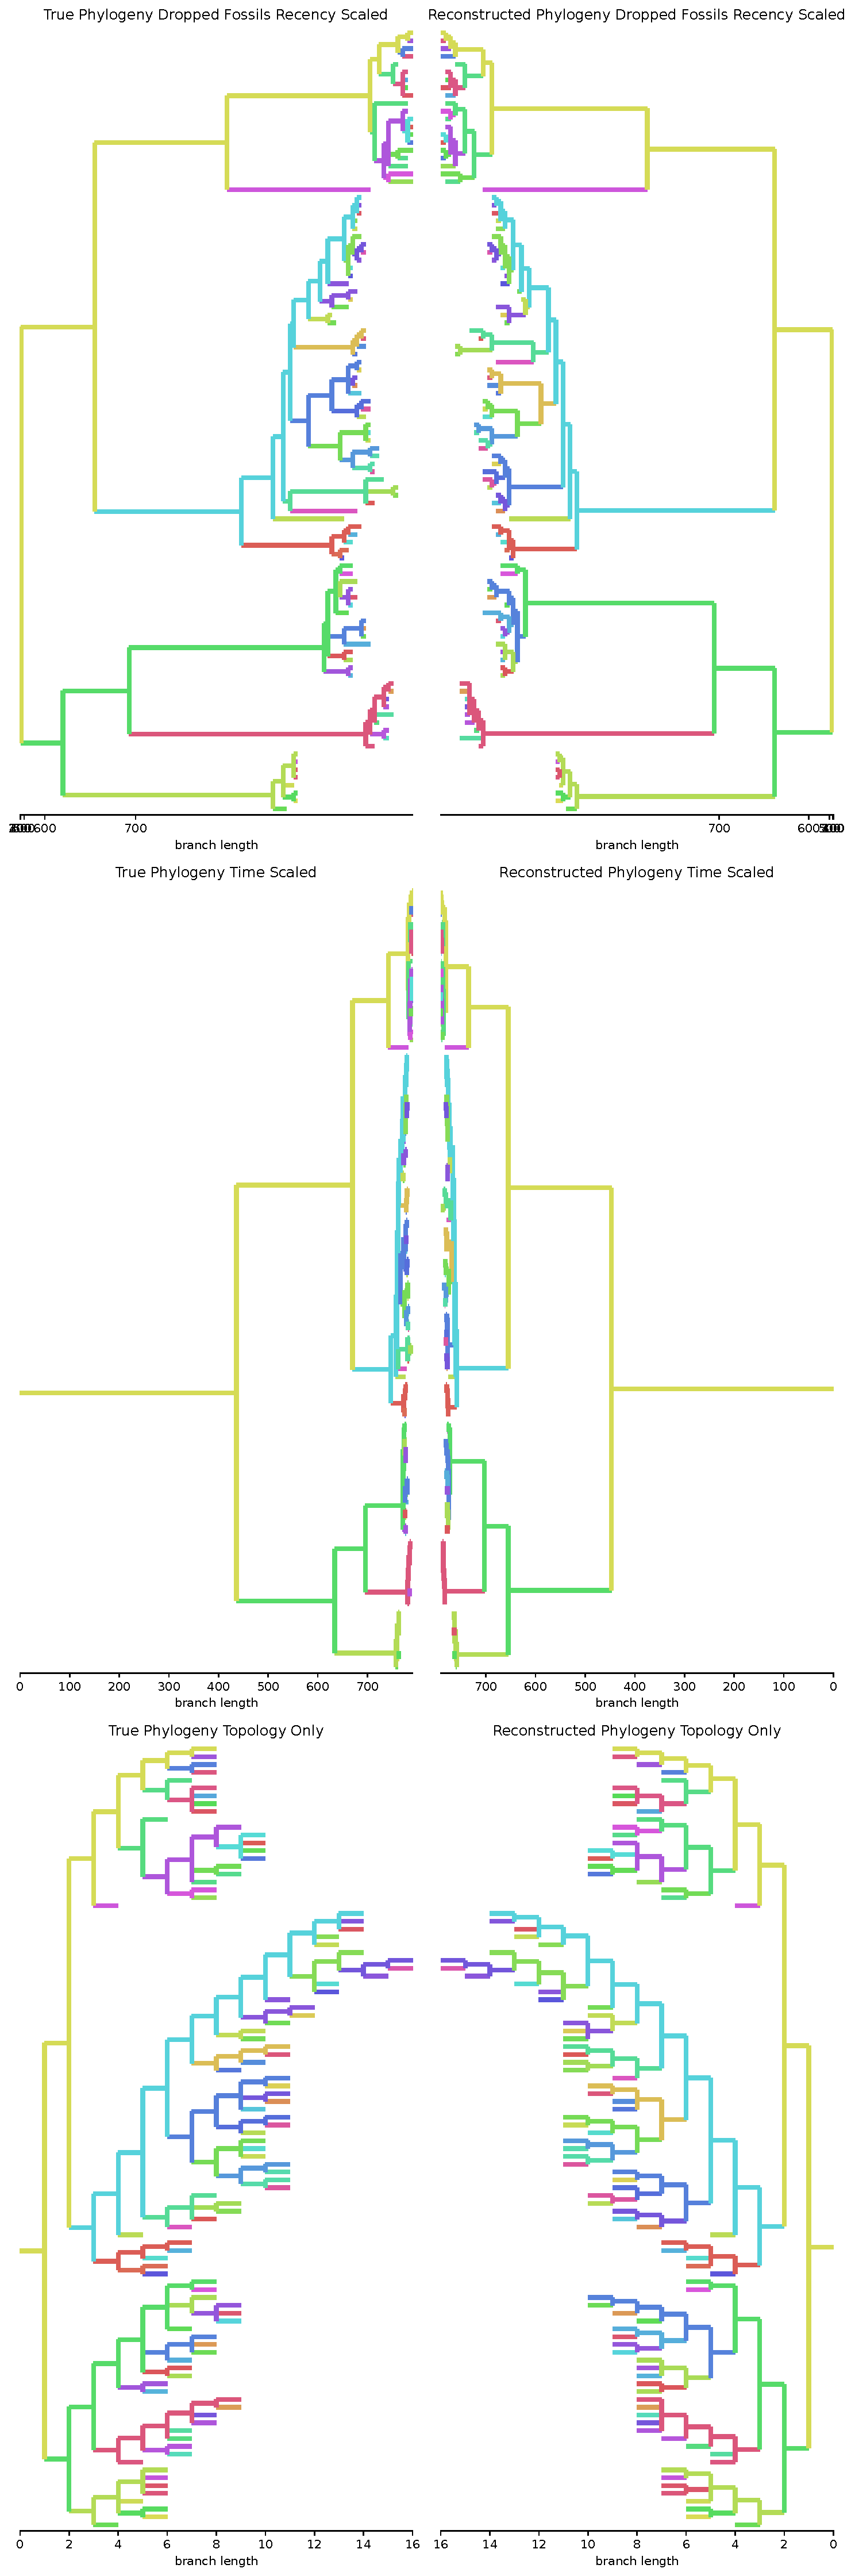
\includegraphics[width=\columnwidth,trim={0 52cm 0 0.8cm},clip]{img/colorclade.pdf}
\caption{\textbf{Sample comparison of true and reconstructed phylogenies.}
\small
Generated using a tilted retention policy and a surface of 32 bits. The true phylogeny is on the left and the reconstructed phylogeny is on the right. Colors are based on a hash from the taxon label for each tip to better facilitate visual comparison. Reconstruction error for this reconstruction was 2.6\%. Visualization created with colorclade \citep{moreno2024colorclade}.
}
\label{fig:colorclade}
\end{figure}


\subsection{More on Microbenchmark Scaling}

We found a positive linear relationship between the speed at which tips were processed with the number of tips already present (i.e. the position of the batch).
However, this was when large outliers are taken into account; by removing them, we see a much more nuanced relationship.
The average-case insertions seem to be increasing up to a certain point, after which they, by and large, taper off in runtime (this pattern is likely due to hardware details enabling faster additions for small trees).
In fact, we found that there was a statistically significant breakpoint through piecewise regression \citep{pilgrim2021piecewise,davies1987hypothesis}.

Given this, we decided on a hardcoded breakpoint of 3 million tips --- that is, when applying piecewise linear regression, we would consider two different lines for the cases where we are under or over 3 million tips.
This hardcoded breakpoint was chosen (as opposed to that generated by the regression) in order to prevent overfitting on a certain model.
Regardless, we found that our chosen breakpoint is also transferable to other instances of reconstruction, such as with a purifying regime --- we see the same pattern of increasing insertion time that begins to taper off past about 3 million tips.

Given this, we then fitted a piecewise linear regression on the data, with a breakpoint at 600 (representing 3 million tips, as batches were of size 5000).
We found that we could not reject the null hypothesis that the the piece corresponding to entries added to a tree with more than 3 million tips had a nonzero slope -- in fact the linear regression modeled it as a negative slope.
For a comparison of simple linear regression with piecewise linear regression on the average case data, see Figure~\ref{fig:average-scaling}.

Regardless, this analysis is merely on the average, and it is very important to take into account the outliers during overall analysis, as they represent the bulk of the work done by the algorithm.

\begin{figure*}[h]
  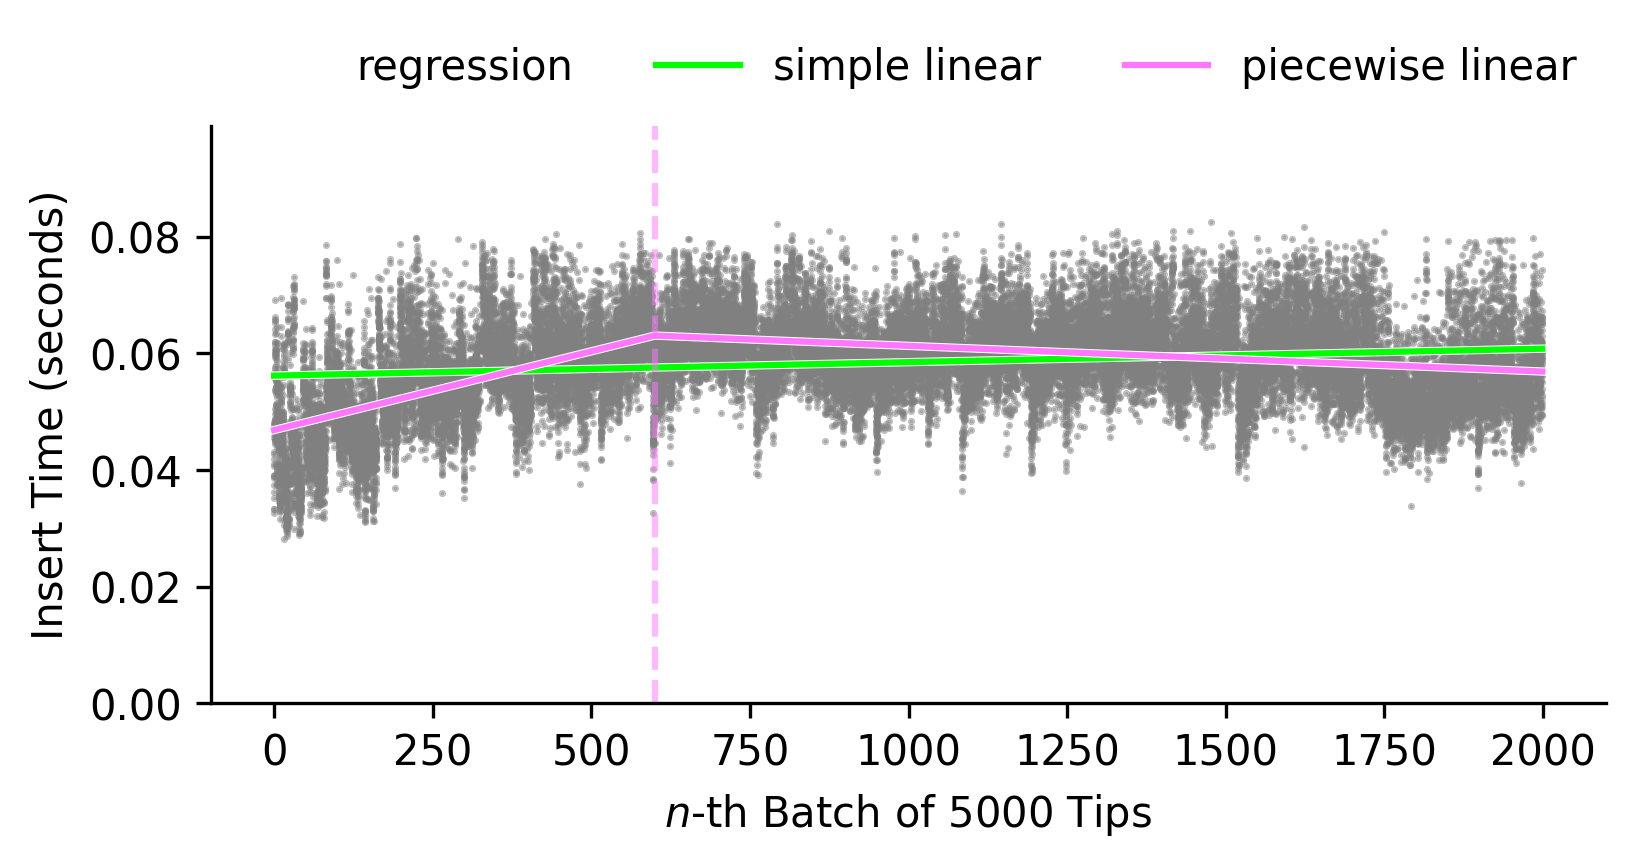
\includegraphics[width=\textwidth]{img/series-average.png}
  \label{fig:average-scaling}
  \caption{\textbf{Time taken per batch with outliers removed.} \small Graph generated by running the same 10 million tip reconstruction 20 times, timing the insertions of each batch of 5000 tips. Breakpoint in piecewise linear regression hardcoded at 3 million tips (i.e. the 600-th batch of 5000 tips).}
\end{figure*}

When measuring the time taken on entire reconstructions with varying numbers of tips, we found an approximately linear relationship between the two variables as depicted in Figure~\ref{fig:asymptotic}. 
This seems to suggest that the outliers detected during the empirical analysis in the main paper are being amortized away by the distance between them. 
However, we can make no conclusive claim without a more thorough analysis.

\begin{figure*}[h]
  \centering
  \begin{minipage}{0.33\textwidth}
    \centering
    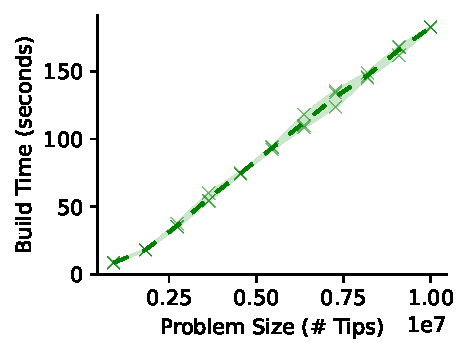
\includegraphics[height=4.3cm]{img/longterm-purifying.pdf}
    \subcaption{Purifying Regime}
    \label{fig:asymptotic:purifying}
  \end{minipage}%
  \begin{minipage}{0.33\textwidth}
    \centering
    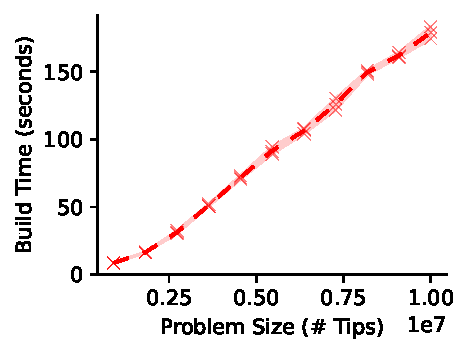
\includegraphics[height=4.3cm,trim={0.7cm 0 0 0},clip]{img/longterm-adaptive.pdf}
    \subcaption{Adaptive Regime}
    \label{fig:asymptotic:adaptive}
  \end{minipage}%
  \begin{minipage}{0.33\textwidth}
    \caption{%
    \textbf{Empirical performance scaling of shortcut table algorithm in microbenchmark trials.} \small
    Panels \ref{fig:asymptotic:purifying} and \ref{fig:asymptotic:adaptive} differ in simulation data source of sampled genomes, with the former exhibiting higher phylogenetic richness. Shaded bands are 100\% percentile intervals, with 3 samples taken per problem size.\vspace{2.5em}
}
    \label{fig:asymptotic}
  \end{minipage}
\end{figure*}


